\documentclass[11pt,a4paper]{article}

% ============================================================
% Guía de usuario LaTeX
% AppImage Launcher Uninstaller
% TECPROG WORLD E.I.R.L.
% Versión con una sola figura general de la GUI
% ============================================================

\usepackage[utf8]{inputenc}
\usepackage[T1]{fontenc}
\usepackage[spanish]{babel}
\usepackage{geometry}
\usepackage{xcolor}
\usepackage{hyperref}
\usepackage{graphicx}
\usepackage{float}
\usepackage{longtable}
\usepackage{array}
\usepackage{booktabs}
\usepackage{fancyhdr}
\usepackage{titlesec}
\usepackage{listings}
\usepackage{enumitem}

\geometry{
    left=2.2cm,
    right=2.2cm,
    top=2.4cm,
    bottom=2.4cm
}

\definecolor{tecgreen}{HTML}{7FB239}
\definecolor{tecdark}{HTML}{111827}
\definecolor{tecgray}{HTML}{374151}
\definecolor{codebg}{HTML}{F3F4F6}
\definecolor{codeborder}{HTML}{CBD5E1}
\definecolor{dangerred}{HTML}{B91C1C}

\hypersetup{
    colorlinks=true,
    linkcolor=tecgreen,
    urlcolor=tecgreen,
    citecolor=tecgreen,
    pdftitle={Guía de usuario de AppImage Launcher Uninstaller},
    pdfauthor={TECPROG WORLD E.I.R.L.}
}

\setlength{\headheight}{14pt}
\pagestyle{fancy}
\fancyhf{}
\lhead{\textbf{TECPROG WORLD E.I.R.L.}}
\rhead{\textbf{AppImage Launcher Uninstaller}}
\cfoot{\thepage}

\titleformat{\section}
{\Large\bfseries\color{tecdark}}
{\thesection}{0.6em}{}

\titleformat{\subsection}
{\large\bfseries\color{tecgray}}
{\thesubsection}{0.6em}{}

\titleformat{\subsubsection}
{\normalsize\bfseries\color{tecgray}}
{\thesubsubsection}{0.6em}{}

\lstset{
    literate=
    {á}{{\'a}}1 {é}{{\'e}}1 {í}{{\'i}}1 {ó}{{\'o}}1 {ú}{{\'u}}1
    {Á}{{\'A}}1 {É}{{\'E}}1 {Í}{{\'I}}1 {Ó}{{\'O}}1 {Ú}{{\'U}}1
    {ñ}{{\~n}}1 {Ñ}{{\~N}}1
    {ü}{{\"u}}1 {Ü}{{\"U}}1
    {¿}{{?`}}1 {¡}{{!`}}1
}

\lstdefinestyle{bashstyle}{
    backgroundcolor=\color{codebg},
    basicstyle=\ttfamily\small,
    breaklines=true,
    frame=single,
    rulecolor=\color{codeborder},
    columns=fullflexible,
    keepspaces=true,
    showstringspaces=false,
    tabsize=4,
    language=bash
}

\lstdefinestyle{textstyle}{
    backgroundcolor=\color{codebg},
    basicstyle=\ttfamily\small,
    breaklines=true,
    frame=single,
    rulecolor=\color{codeborder},
    columns=fullflexible,
    keepspaces=true,
    showstringspaces=false,
    tabsize=4
}

\begin{document}

\begin{titlepage}
    \centering
    \vspace*{1.2cm}

    {\Huge\bfseries\color{tecdark} Guía de usuario de AppImage Launcher Uninstaller\par}

    \vspace{0.5cm}
    {\Large Desinstalación segura de lanzadores AppImage y recursos locales en Linux Mint\par}

    \vspace{1.0cm}
    {\large Linux Mint \quad | \quad AppImage \quad | \quad Tkinter \quad | \quad XDG Desktop Entry \quad | \quad 2026\par}

    \vfill

    \begin{tabular}{>{\bfseries}p{5.0cm}p{9.5cm}}
        Empresa & TECPROG WORLD E.I.R.L. \\
        RUC & 20608743252 \\
        Tipo de contribuyente & Empresa Individual de Responsabilidad Limitada \\
        Estado del contribuyente & Activo \\
        Condición del contribuyente & Habido \\
        Domicilio fiscal & Mza. C Lote 43 Urb. Los Nísperos, San Martín de Porres, Lima, Lima \\
        Actividad principal & 7110 -- Actividades de arquitectura e ingeniería y actividades conexas de consultoría técnica \\
        Sitio web & \url{https://tecprog-world-store.github.io/} \\
    \end{tabular}

    \vfill
    {\large Documento técnico para administración local de aplicaciones portables, accesos de menú y recursos gráficos asociados.\par}

    \vspace{0.8cm}
    {\large \today\par}
\end{titlepage}

\tableofcontents
\newpage

\section{Organización de archivos para compilar esta guía}

Para incorporar la captura de pantalla del programa en el PDF, se recomienda trabajar con esta estructura:

\begin{lstlisting}[style=textstyle]
GuiaAppImageLauncher/
|-- guia_usuario_appimage_launcher_uninstaller.tex
|-- figuras/
    |-- appimage_launcher_uninstaller_01.png
\end{lstlisting}

La figura \texttt{appimage\_launcher\_uninstaller\_01.png} debe contener la interfaz completa del software, incluyendo la lista de lanzadores, el panel de detalles, las opciones de desinstalación y los botones principales. Esta guía queda preparada para trabajar con una sola figura general, ya que dicha captura resume el flujo completo de uso.

\begin{lstlisting}[style=bashstyle]
pdflatex guia_usuario_appimage_launcher_uninstaller.tex
pdflatex guia_usuario_appimage_launcher_uninstaller.tex
\end{lstlisting}

\section{Objetivo del software}

\textit{AppImage Launcher Uninstaller} es una aplicación gráfica desarrollada en Python con Tkinter para desinstalar lanzadores locales asociados a aplicaciones \texttt{AppImage}. Su objetivo es eliminar de forma ordenada el archivo \texttt{.desktop}, el ejecutable portable almacenado en \texttt{\$HOME/.local/opt} y el ícono asociado dentro de \texttt{\$HOME/.local/share/icons}. La herramienta complementa a \textit{AppImage Launcher Creator}, ya que permite revertir la instalación local sin borrar recursos globales del sistema.

\section{Problema que resuelve}

Cuando un usuario crea lanzadores para aplicaciones \texttt{AppImage}, el sistema suele generar varios recursos locales. Estos recursos pueden quedar dispersos en carpetas como \texttt{.local/share/applications}, \texttt{.local/share/icons} y \texttt{.local/opt}. Si el usuario elimina solo el archivo \texttt{AppImage}, pueden quedar accesos rotos en el menú; si elimina solo el lanzador, pueden quedar ejecutables e íconos ocupando espacio de forma innecesaria.

\section{Alcance seguro de eliminación}

La herramienta fue diseñada con un criterio de seguridad conservador. Por defecto, solo elimina archivos ubicados dentro del perfil del usuario y evita modificar rutas globales del sistema.

\begin{longtable}{>{\bfseries}p{6cm}p{8cm}}
\toprule
Recurso & Ruta gestionada \\
\midrule
Lanzadores de usuario & \texttt{\$HOME/.local/share/applications/*.desktop} \\
Ejecutables AppImage locales & \texttt{\$HOME/.local/opt/<id>/} \\
Íconos locales & \texttt{\$HOME/.local/share/icons/} \\
Recursos globales del sistema & No se eliminan en esta versión \\
\bottomrule
\end{longtable}

\section{Requisitos del sistema}

Para ejecutar el programa se requiere:

\begin{itemize}[leftmargin=1.2cm]
    \item Linux Mint, Ubuntu, Debian o una distribución compatible.
    \item Python 3.
    \item Tkinter.
    \item Lanzadores \texttt{.desktop} previamente creados para aplicaciones AppImage.
\end{itemize}

Si Tkinter no está disponible, instalarlo con:

\begin{lstlisting}[style=bashstyle]
sudo apt update
sudo apt install python3-tk
\end{lstlisting}

\section{Ejecución del programa}

Si se ejecuta directamente desde el archivo Python:

\begin{lstlisting}[style=bashstyle]
python3 appimage_launcher_uninstaller.py
\end{lstlisting}

Si tiene permisos de ejecución:

\begin{lstlisting}[style=bashstyle]
chmod +x appimage_launcher_uninstaller.py
./appimage_launcher_uninstaller.py
\end{lstlisting}

Si fue instalado mediante paquete \texttt{.deb}, puede abrirse desde terminal con:

\begin{lstlisting}[style=bashstyle]
appimage-launcher-uninstaller
\end{lstlisting}

También puede buscarse en el menú de aplicaciones como:

\begin{lstlisting}[style=textstyle]
AppImage Launcher Uninstaller
\end{lstlisting}

\section{Descripción general de la interfaz}

La interfaz se organiza en dos paneles principales. El panel izquierdo lista los lanzadores AppImage detectados en el perfil del usuario. El panel derecho muestra los detalles técnicos del lanzador seleccionado y permite configurar qué recursos serán eliminados. En la figura \ref{fig:uninstaller-principal} se observa la interfaz completa de la herramienta, por lo que esta única captura permite identificar los componentes principales del flujo de desinstalación.

\begin{figure}[H]
    \centering
    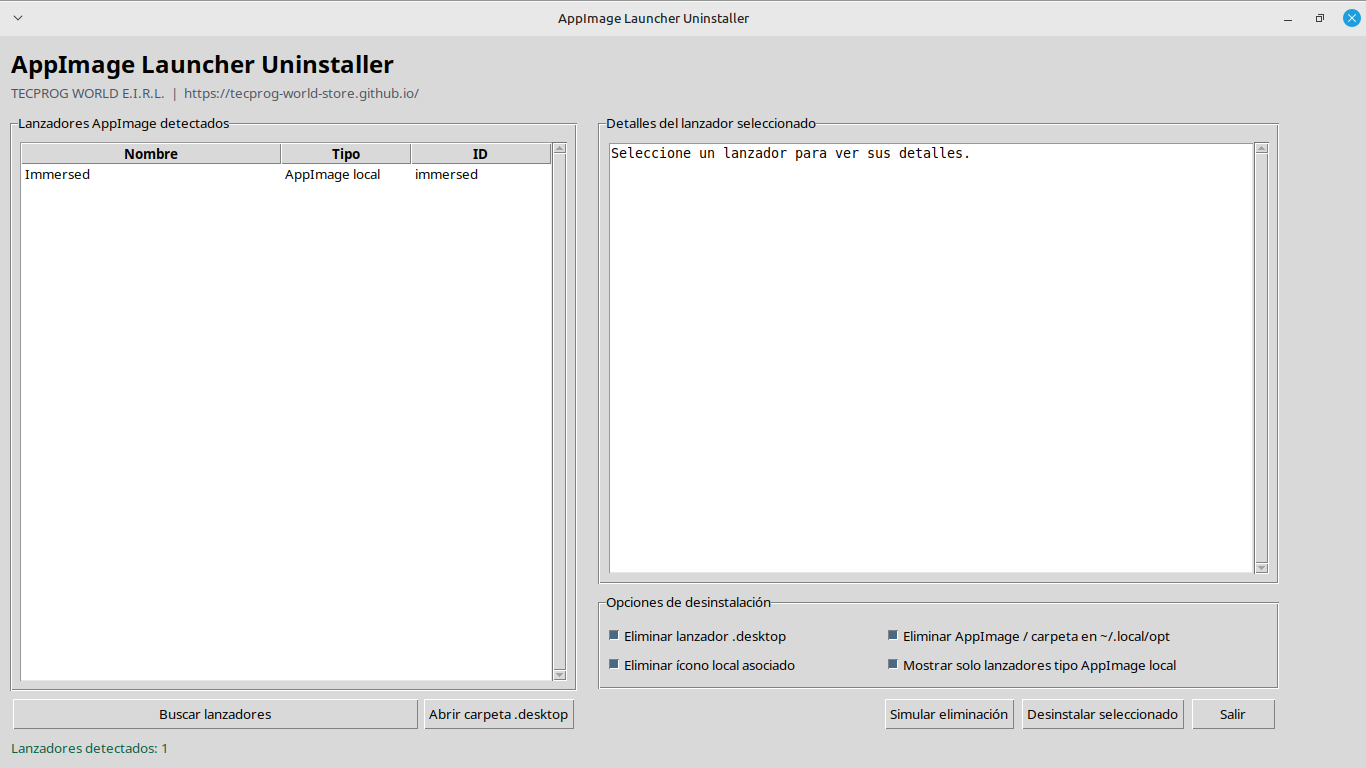
\includegraphics[width=0.98\textwidth]{figuras/appimage_launcher_uninstaller_01.png}
    \caption{Interfaz completa de AppImage Launcher Uninstaller con listado de lanzadores, panel de detalles, opciones de eliminación y botones de acción.}
    \label{fig:uninstaller-principal}
\end{figure}

\section{Panel de lanzadores detectados}

El panel izquierdo muestra los lanzadores encontrados dentro de:

\begin{lstlisting}[style=textstyle]
~/.local/share/applications/
\end{lstlisting}

La herramienta analiza cada archivo \texttt{.desktop} y revisa el campo \texttt{Exec}. Si el ejecutable apunta a un archivo con extensión \texttt{.AppImage}, el programa lo identifica como un lanzador relacionado con AppImage. En la figura \ref{fig:uninstaller-principal}, este panel corresponde a la zona izquierda donde aparecen las aplicaciones detectadas.

\subsection{Tipos detectados}

\begin{longtable}{>{\bfseries}p{5cm}p{9cm}}
\toprule
Tipo & Descripción \\
\midrule
AppImage local & El ejecutable está dentro de \texttt{\$HOME/.local/opt}. Es el caso más seguro de eliminar. \\
AppImage externo & El ejecutable apunta a un archivo AppImage fuera de \texttt{\$HOME/.local/opt}. La herramienta puede mostrarlo, pero no borra archivos externos por seguridad. \\
Otro & El lanzador no corresponde claramente a una aplicación AppImage. \\
\bottomrule
\end{longtable}

\section{Panel de detalles}

Al seleccionar un lanzador, el programa muestra información técnica como:

\begin{itemize}[leftmargin=1.2cm]
    \item Nombre visible.
    \item ID del lanzador.
    \item Tipo detectado.
    \item Ruta del archivo \texttt{.desktop}.
    \item Línea \texttt{Exec}.
    \item Ruta del ejecutable detectado.
    \item Directorio de instalación en \texttt{\$HOME/.local/opt}.
    \item Ícono asociado.
    \item Categorías del menú.
    \item Plan de eliminación según las opciones activas.
\end{itemize}

Este panel permite revisar de forma técnica qué se eliminará antes de ejecutar la operación. En la figura \ref{fig:uninstaller-principal}, el panel de detalles se ubica en la zona derecha de la ventana.

\section{Opciones de desinstalación}

La interfaz permite activar o desactivar tres acciones principales.

\subsection{Eliminar lanzador \texttt{.desktop}}

Esta opción elimina el acceso del menú de aplicaciones:

\begin{lstlisting}[style=textstyle]
~/.local/share/applications/<id>.desktop
\end{lstlisting}

Debe mantenerse activada si se desea que la aplicación desaparezca del menú.

\subsection{Eliminar AppImage o carpeta en \texttt{\~{}/.local/opt}}

Esta opción elimina el ejecutable y la carpeta de instalación local:

\begin{lstlisting}[style=textstyle]
~/.local/opt/<id>/
\end{lstlisting}

Por seguridad, la herramienta solo elimina carpetas dentro de \texttt{\$HOME/.local/opt}. No borra AppImages ubicados en \texttt{Descargas}, \texttt{Documentos} u otras rutas externas.

\subsection{Eliminar ícono local asociado}

Esta opción elimina el ícono asociado si se encuentra dentro de:

\begin{lstlisting}[style=textstyle]
~/.local/share/icons/
\end{lstlisting}

No elimina íconos globales ubicados en \texttt{/usr/share/icons}.

\subsection{Mostrar solo lanzadores tipo AppImage local}

Esta opción filtra la lista para mostrar solo lanzadores que la herramienta considera relacionados con AppImage. Es útil para evitar modificar accidentalmente lanzadores de otras aplicaciones.

\section{Botones principales}

\subsection{Buscar lanzadores}

Actualiza la lista de lanzadores detectados. Debe usarse después de instalar o eliminar aplicaciones AppImage.

\subsection{Abrir carpeta \texttt{.desktop}}

Abre la carpeta local donde están los lanzadores del usuario:

\begin{lstlisting}[style=textstyle]
~/.local/share/applications/
\end{lstlisting}

\subsection{Simular eliminación}

Muestra una vista previa de los archivos y carpetas que serían eliminados, sin borrar nada. Se recomienda usar este botón antes de ejecutar la desinstalación real.

\subsection{Desinstalar seleccionado}

Elimina los recursos seleccionados después de una confirmación explícita del usuario. Esta acción no se puede deshacer automáticamente.

\subsection{Salir}

Cierra la aplicación.

\section{Ejemplo de desinstalación de Immersed}

Supóngase que Immersed fue instalado como AppImage local mediante \textit{AppImage Launcher Creator}. La estructura esperada sería:

\begin{lstlisting}[style=textstyle]
/home/pc/.local/opt/immersed/
|-- immersed.AppImage

/home/pc/.local/share/icons/
|-- immersed.png

/home/pc/.local/share/applications/
|-- immersed.desktop
\end{lstlisting}

El procedimiento recomendado es:

\begin{enumerate}[leftmargin=1.2cm]
    \item Abrir \textit{AppImage Launcher Uninstaller}.
    \item Presionar \textbf{Buscar lanzadores}.
    \item Seleccionar \textbf{Immersed}.
    \item Revisar el panel de detalles.
    \item Presionar \textbf{Simular eliminación}.
    \item Confirmar que las rutas corresponden a \texttt{immersed}.
    \item Presionar \textbf{Desinstalar seleccionado}.
    \item Confirmar la operación.
\end{enumerate}

\section{Verificación desde terminal}

Después de desinstalar, se puede verificar que el lanzador ya no existe:

\begin{lstlisting}[style=bashstyle]
ls -lh ~/.local/share/applications/immersed.desktop
\end{lstlisting}

Si fue eliminado correctamente, el sistema indicará que el archivo no existe. También puede verificarse la carpeta de instalación:

\begin{lstlisting}[style=bashstyle]
ls -lh ~/.local/opt/immersed
\end{lstlisting}

Y el ícono:

\begin{lstlisting}[style=bashstyle]
ls -lh ~/.local/share/icons/immersed.png
\end{lstlisting}

\section{Actualización del menú de aplicaciones}

Después de eliminar un lanzador, la herramienta intenta actualizar la base de datos de aplicaciones. Si el menú no se refresca inmediatamente, puede ejecutarse:

\begin{lstlisting}[style=bashstyle]
update-desktop-database ~/.local/share/applications
\end{lstlisting}

En XFCE también puede reiniciarse el panel:

\begin{lstlisting}[style=bashstyle]
xfce4-panel -r
\end{lstlisting}

Otra opción es cerrar sesión y volver a ingresar.

\section{Instalación mediante paquete \texttt{.deb}}

Para construir el paquete \texttt{.deb}, se utiliza el script:

\begin{lstlisting}[style=bashstyle]
chmod +x build_appimage_launcher_uninstaller_deb.sh
./build_appimage_launcher_uninstaller_deb.sh
\end{lstlisting}

El archivo generado se ubicará en:

\begin{lstlisting}[style=textstyle]
dist/appimage-launcher-uninstaller_0.1.0_all.deb
\end{lstlisting}

Para instalarlo:

\begin{lstlisting}[style=bashstyle]
sudo apt install ./dist/appimage-launcher-uninstaller_0.1.0_all.deb
\end{lstlisting}

Para desinstalar la propia herramienta:

\begin{lstlisting}[style=bashstyle]
sudo apt remove appimage-launcher-uninstaller
\end{lstlisting}

\section{Archivos instalados por el paquete \texttt{.deb}}

La instalación mediante \texttt{.deb} coloca archivos en rutas globales administradas por el sistema:

\begin{lstlisting}[style=textstyle]
/usr/lib/appimage-launcher-uninstaller/appimage_launcher_uninstaller.py
/usr/bin/appimage-launcher-uninstaller
/usr/share/applications/appimage-launcher-uninstaller.desktop
/usr/share/icons/hicolor/256x256/apps/appimage-launcher-uninstaller.png
/usr/share/doc/appimage-launcher-uninstaller/
\end{lstlisting}

Estos recursos corresponden a la herramienta desinstaladora, no a las aplicaciones AppImage gestionadas por ella.

\section{Buenas prácticas}

\begin{itemize}[leftmargin=1.2cm]
    \item Usar siempre \textbf{Simular eliminación} antes de desinstalar.
    \item Revisar que las rutas del plan correspondan a la aplicación correcta.
    \item Mantener activado el filtro de lanzadores AppImage para reducir riesgos.
    \item No eliminar manualmente archivos si no se reconoce su función.
    \item Realizar pruebas con aplicaciones no críticas antes de usar la herramienta en flujos de trabajo principales.
\end{itemize}

\section{Limitaciones conocidas}

La herramienta no elimina recursos instalados de forma global por paquetes \texttt{.deb}, \texttt{Flatpak}, \texttt{Snap} o gestores de paquetes del sistema. Tampoco elimina configuraciones internas creadas por cada aplicación dentro de carpetas como \texttt{\$HOME/.config}, porque estas rutas pueden contener datos de usuario que requieren una decisión explícita. En futuras versiones se puede incorporar una opción avanzada para detectar configuraciones residuales, pero debe implementarse con confirmaciones adicionales.

\section{Conclusión}

\textit{AppImage Launcher Uninstaller} permite administrar de forma segura los recursos locales creados para aplicaciones AppImage. La herramienta elimina lanzadores, ejecutables locales e íconos asociados sin intervenir en rutas globales del sistema, lo cual reduce el riesgo de borrar archivos críticos. Este enfoque complementa el flujo de instalación de \textit{AppImage Launcher Creator} y permite a TECPROG WORLD E.I.R.L. disponer de una pequeña suite de utilidades para integrar y retirar aplicaciones portables en Linux Mint.

\section*{Contacto institucional}

\begin{longtable}{>{\bfseries}p{5cm}p{10cm}}
Empresa & TECPROG WORLD E.I.R.L. \\
RUC & 20608743252 \\
Actividad principal & Actividades de arquitectura e ingeniería y actividades conexas de consultoría técnica \\
Ubicación & San Martín de Porres, Lima, Perú \\
Sitio web & \url{https://tecprog-world-store.github.io/} \\
\end{longtable}

\end{document}
